\hypertarget{chapter2-ux69cbux6587ux89e3ux6790ux306eux57faux672c}{%
\chapter{構文解析の基本}\label{chapter2-ux69cbux6587ux89e3ux6790ux306eux57faux672c}}
\index{こうぶんかいせき@構文解析!基本}
\index{さんじゅつしき@算術式}

この章からいよいよ構文解析についての説明を始めたいと思います。とはいっても本書を手に取った皆様は構文解析についてまだ馴染みがないかと思います。そこで、まずは簡単な算術式の構文解析を例にして、構文解析の基本について学ぶことにしましょう。

算術式という言い方は堅苦しいですが、要は数式のことです。たとえば、\texttt{1\ +\ 2}や\texttt{(1\ +\ 2)\ *\ 3}、\texttt{(3\ *\ 3)\ *\ (2\ *\ 3)}のようなものです。プログラマーの皆さんなら普段、日常的にプログラムの一部として算術式を書いているでしょう。算術式は非常にシンプルな「言語」なので、構文解析の題材にするのに最適なのです。

\hypertarget{chapter2-ux7b97ux8853ux5f0fux306eux6587ux6cd5}{%
\section{算術式の文法}\label{chapter2-ux7b97ux8853ux5f0fux306eux6587ux6cd5}}
\index{さんじゅつしき@算術式!文法}
\index{じくかいせき@字句解析}
\index{とーくん@トークン}
\index{けいしきぶんぽう@形式文法}

ただ「算術式」といっただけだと人によってかなりイメージするものが異なります。本書では以下の条件を満たすものを算術式とします。

\begin{itemize}
\tightlist
\item
  四則演算ができる

  \begin{itemize}
  \tightlist
  \item
    足し算は\texttt{x+y}
  \item
    引き算は\texttt{x-y}
  \item
    掛け算は\texttt{x*y}
  \item
    割り算は\texttt{x/y}
  \end{itemize}
\item
  優先順位は掛け算・割り算が高く、足し算・引き算が低い

  \begin{itemize}
  \tightlist
  \item
    \texttt{1+2*3}は\texttt{1+(2*3)}と解釈される
  \item
    \texttt{7-6/2}は\texttt{7-(6/2)}と解釈される
  \end{itemize}
\item
  掛け算・割り算の優先順位は同じで、足し算・引き算の優先順位も同じ
\item
  優先順位が同じ演算子は左から右に結びつく

  \begin{itemize}
  \tightlist
  \item
    \texttt{1+2-3}は\texttt{(1+2)-3}と解釈される
  \end{itemize}
\item
  値は整数のみ

  \begin{itemize}
  \tightlist
  \item
    \texttt{1+2.0}のような式はエラーになる
  \end{itemize}
\item
  式の優先順位を変えるために括弧を使うことができる

  \begin{itemize}
  \tightlist
  \item
    \texttt{1+2*3}は\texttt{1+(2*3)}の意味になるが、\texttt{(1+2)*3}と書くことで意味が変わる
  \end{itemize}
\item
  スペースは使えない

  \begin{itemize}
  \tightlist
  \item
    \texttt{1+2}はOKだが、\texttt{1\ +\ 2}はエラーになる
  \end{itemize}
\end{itemize}

最後の「スペースは使えない」という制限はあくまで単純化のためです。特に、字句解析（文字列を意味のある単位、トークンに分割する処理）を単純化し、構文解析の核となる考え方に集中するために設けています。実際の算術式ではスペースも使えて無視されるのが一般的ですが、その処理は後の章で触れることにします。

この定義に従う算術式には以下のようなものが含まれます。

\begin{verbatim}
100  # 100
1+2*3  # 7
(1+2)*3  # 9
3*(1+2)  # 9
12/3  # 4
1+3*4/2  # 7
\end{verbatim}

皆さんは何かしらのプログラミング言語を使ってプログラムを書いているはずですから、上のような算術式は馴染みが深いはずです。

しかし、上のような日本語を使った定義だけでは算術式の文法を表現するのには不十分です。たとえば「式の優先順位を変えるために括弧を使うことができる」といっても、なんとなくはわかるものの、定義としては曖昧です。もちろん、日本語で詳しく記述して曖昧さを少なくしていくこともできますが、いたずらに長くなるだけです。

曖昧さがない形で文法を表現するために、特別な記法を使うことが一般的です。これを\textbf{形式文法}と呼びます。「形式文法」という名前は堅苦しく聞こえるかもしれませんが、要は「プログラミング言語の文法を書くための、決まった書き方」のことです。

たとえば、皆さんがJavaのメソッドを書く時にも決まった形式があるように（例：\texttt{public\ void\ methodName()\ \{\ ...\ \}}）、プログラミング言語の文法そのものを記述する時にも決まった形式があるのです。

次節では、そのような形式文法の中でも最も広く使われているBNF（Backus-Naur
Form、バッカス・ナウア記法）を使って、算術式の文法を表現してみましょう。BNFは、プログラミング言語の仕様書やドキュメントでよく見かける記法です。

\hypertarget{chapter2-ux7b97ux8853ux5f0fux306ebnf}{%
\section{算術式のBNF}\label{chapter2-ux7b97ux8853ux5f0fux306ebnf}}
\index{BNF}
\index{EBNF}
\index{めたぶんぽう@メタ文法}

プログラミング言語の文法自体を表現する文法（メタ文法といいます）の一つに、BNFがあります。BNFは、プログラミング言語の文法をはじめ、インターネット上でのメッセージ交換フォーマットなど、様々な文法を表現するのに使われています。本書の読者の方にはBNFに馴染みのない方も多いと思うので、算術式のBNFの前にBNFについて説明します。本書では、記述を簡潔にするため、ISO/IEC
14977で仕様が策定されたEBNF\footnote{翻訳: ISO/IEC 14977:1996
  Information technology --- Syntactic metalanguage --- Extended BNF
  https://hazm.at/mox/lang/meta-language/ebnf/iso-iec-14977-extended-bnf/index.html}で用いられる繰り返し（\texttt{\{\}}）、オプション（\texttt{{[}{]}}）、グループ化（\texttt{()}）といった拡張記法を一部取り入れ、これを広義のBNFとして扱います。なお、Java言語仕様など多くの仕様書でも、この種の拡張BNFが一般的に用いられています。BNFには歴史的に多くの方言が存在するため、本書で用いる記法について事前に説明しておきます。

\hypertarget{chapter2-bnfux306eux6982ux8981}{%
\subsection{BNFの概要}\label{chapter2-bnfux306eux6982ux8981}}

BNFはFortranの開発者でもある、John
Backus（ジョン・バッカス）らが開発した記法です。BNFは「プログラミング言語」そのものの文法を記述するために開発されました。基本情報技術者試験でも出題されるので、そこで知った方もおられるかもしれません。

本書で用いる広義のBNF（EBNFの要素を取り入れたもの）の主要な記法は以下の通りです。

\begin{itemize}
\tightlist
\item
  \texttt{=} :
  左辺の記号（厳密には非終端記号。詳しくは後述）と右辺の定義を区切ります。
\item
  \texttt{;} :
  文法規則の終端を示します（各規則はセミコロンで終わります）。
\item
  並び（連接）: 本書では \texttt{A\ B}
  のようにスペースで表します（ISO/IECのEBNFでは \texttt{A,\ B}
  のようにカンマで表すのが標準です）。
\item
  \texttt{\textbar{}} : 選択を表します。例えば \texttt{A\ \textbar{}\ B}
  は「AまたはB」を意味します。
\item
  \texttt{\{\}} : 0回以上の繰り返しを表します。例えば \texttt{A\ \{B\}}
  は「Aの後にBが0回以上続く」ことを意味します。
\item
  \texttt{{[}{]}} : 0回または1回の出現（オプション）を表します。例えば
  \texttt{{[}A{]}\ B}
  は「Aがあるかもしれないし、ないかもしれないが、その後にBが続く」ことを意味します。
\item
  \texttt{()} : グループ化を表します。例えば
  \texttt{(A\ \textbar{}\ B)\ C}
  は「AまたはBの後にCが続く」ことを意味します。
\item
  \texttt{\textquotesingle{}...\textquotesingle{}} または
  \texttt{"}\ldots{}\texttt{"} : 終端記号（リテラル文字列）を表します。
\item
  非終端記号（例: \texttt{expr}, \texttt{term}）:
  他の規則で定義される記号を表します（用語の詳細は後述します）。
\end{itemize}

では早速、BNFの具体例を見て行きましょう。以下の例は2.1で出てきた算術式を元に、

\begin{itemize}
\tightlist
\item
  扱える数値は一桁だけ
\end{itemize}

のように単純化したBNFです。

\begin{verbatim}
expr = term { ('+' | '-') term };
term = factor { ('*' | '/') factor };
factor = NUMBER | '(' expr ')';
NUMBER = '0' | '1' | '2' | '3' | '4' | '5' | '6' | '7' | '8' | '9';
\end{verbatim}

たくさんの記号が出てきて戸惑われたかもしれませんが、一つずつ丁寧に見ていきましょう。

\hypertarget{chapter2-expr}{%
\subsection{expr}\label{chapter2-expr}}

BNFでは、以下のような\textbf{生成規則}の集まりによって、文法を表現します。

\begin{verbatim}
expr = term { ('+' | '-') term };
\end{verbatim}

\texttt{=}の左側である\texttt{expr}が\textbf{左辺}（この規則で定義される非終端記号）で、右側が\textbf{右辺}（その定義）になります。

ここでは

\begin{verbatim}
term { ('+' | '-' ) term }
\end{verbatim}

が本体になります。

本体の中に出てくる、他の規則を参照する部分（ここでは\texttt{term})を\textbf{非終端記号}と呼びます（この用語は前にも登場しましたが、ここで正式に定義します）。これは「まだ展開の余地がある記号」という意味で、同じBNF内で定義されている他の非終端記号と一致する必要があります。Javaでいえば、メソッド呼び出しのようなものです。

一方、\texttt{\textquotesingle{}+\textquotesingle{}}や\texttt{\textquotesingle{}-\textquotesingle{}}のように\texttt{\textquotesingle{}}で囲まれた記号や文字を\textbf{終端記号}と呼びます。これは「これ以上展開できない、最終的な文字」という意味で、実際にプログラムに書かれる文字そのものを表します。Javaでいえば、\texttt{+}演算子や\texttt{;}セミコロンのようなものです。

BNFにおいて\texttt{\{\}}で囲まれたものは、その中の要素が0回以上繰り返して出現することを示しています。したがって、

\begin{verbatim}
term { ('+' | '-') term }
\end{verbatim}

という記述は、まず\texttt{term}が出現し、その後に「\texttt{+}または\texttt{-}とそれに続く\texttt{term}」が0回以上繰り返して出現することを示しています。0回以上という言い方が重要です。というのは、\texttt{term}が1回だけ出現してその後は何も出現しない場合もあるからです。たとえば、\texttt{1}という式はこの規則にマッチしますが、\texttt{\{\}}で囲まれた部分は出現していません。

この生成規則を日本語で表現すると「\texttt{expr}という非終端記号は、右辺の定義
\texttt{term\ \{\ (\textquotesingle{}+\textquotesingle{}\ \textbar{}\ \textquotesingle{}-\textquotesingle{})\ term\ \}}
によって定義される」と読むことができます。

なお、本来の（ISO/IEC）BNFでは

\begin{verbatim}
expr = term, { ('+' | '-'), term };
\end{verbatim}

のように要素間をカンマで区切りますが、本書では可読性を考慮してスペースで区切るようにしています。

\hypertarget{chapter2-term}{%
\subsection{term}\label{chapter2-term}}

\texttt{term}
は算術式の中で、掛け算や割り算を含んだ式を表す規則です。\texttt{factor}という規則を参照しています。

\begin{verbatim}
term = factor { ('*' | '/') factor };
\end{verbatim}

この規則によって\texttt{term}は、\texttt{factor}が\texttt{*}または\texttt{/}を挟んで0回以上繰り返して出現することを示しています。

\hypertarget{chapter2-factor}{%
\subsection{factor}\label{chapter2-factor}}

\texttt{factor}は算術式の中で、数値や括弧で囲まれた式を表す規則です。

\begin{verbatim}
factor = NUMBER | '(' expr ')';
\end{verbatim}

この規則によって\texttt{factor}は、

\begin{itemize}
\tightlist
\item
  \texttt{NUMBER}
\item
  \texttt{(}と\texttt{)}に挟まれた\texttt{expr}
\end{itemize}

のどちらかであることを示しています。

\hypertarget{chapter2-number}{%
\subsection{NUMBER}\label{chapter2-number}}

\texttt{NUMBER}は数値を表す規則です。ここでは単純化のために1桁の整数のみを扱っています。

\begin{verbatim}
NUMBER = '0' | '1' | '2' | '3' | '4' | '5' | '6' | '7' | '8' | '9';
\end{verbatim}

\texttt{NUMBER}は\texttt{0}から\texttt{9}のどれか1文字であることを示しています。

\hypertarget{chapter2-bnfux3092ux4f7fux3063ux305fux89e3ux6790ux30d7ux30edux30bbux30b9}{%
\section{BNFを使った解析プロセス}\label{chapter2-bnfux3092ux4f7fux3063ux305fux89e3ux6790ux30d7ux30edux30bbux30b9}}

算術式の文法を規則\texttt{expr}を含むBNFによって表現することができました。この記述には\textbf{曖昧さがなく}、スペースを許さないことや演算子の優先順位などの概念も含まれています。

この規則\texttt{expr}を使うと、式\texttt{1+2}はどのように解析できるのでしょうか？ここでは、その概要について簡単に説明します。

このBNFを使って解析を行う方法は一意ではなく、様々なやり方（手続き）があります。その個々の手続きがまさに構文解析アルゴリズムとなります。個々の構文解析アルゴリズムについては第5章で詳しく説明しますが、ここでは、BNFを使って\textbf{素直に}算術式を解析する方法の概要を説明します。ちなみに、構文解析に限った話ではありませんが、そのような\textbf{素直な}方法のことをナイーブ（naive）な方法と呼ぶことがあります。

まず最初にBNFの規則を関数とみなします。たとえば、規則\texttt{expr}は関数\texttt{expr}に対応し、規則\texttt{term}は関数\texttt{term}に対応します。これらの規則に対応する関数は、解析したい文字列を引数に取り、解析の結果を返します。

この関数の宣言をJavaライクな擬似コードで表すと、以下のようになります。

\begin{Shaded}
\begin{Highlighting}[]
\NormalTok{ParseResult }\FunctionTok{expr}\NormalTok{(}\BuiltInTok{String}\NormalTok{ input);}
\end{Highlighting}
\end{Shaded}

次に関数の呼び出しを構文解析とみなします。引数として解析したい文字列を渡すと、構文解析結果が返ってくるものとします。

たとえば、\texttt{expr("1+2")}という関数呼び出しは、文字列\texttt{"1+2"}を解析することを示します。まだ\texttt{expr}の本体がありませんが、結果としては、解析が成功した旨の情報がかえってきて欲しいでしょう。一方、\texttt{expr("1+")}という関数呼び出しは、解析が失敗した旨の情報がかえってきて欲しいはずです。

関数の呼び出し結果は、

\begin{itemize}
\tightlist
\item
  解析に成功した場合：成功したことを表す情報と、まだ解析していない残りの文字列。これを\texttt{(SUCCESS,\ remaining\_string)}と表す
\item
  失敗した場合：失敗を表す定数\texttt{FAIL}を返す
\end{itemize}

のどちらかであるとします。

以上の前提を元に、実際に\texttt{expr("1+2")}がどのように解析されるか、主要なポイントを追ってみましょう。詳細な内部動作は省略し、重要な部分に焦点を当てて説明します。

\hypertarget{chapter2-ux89e3ux6790ux306eux6d41ux308c}{%
\subsection{解析の流れ}\label{chapter2-ux89e3ux6790ux306eux6d41ux308c}}

\texttt{expr("1+2")}の解析がどのように進むか、主要なポイントを見てみましょう：

\begin{enumerate}
\def\labelenumi{\arabic{enumi}.}
\tightlist
\item
  最初の数字「1」の解析
\end{enumerate}

\begin{itemize}
\tightlist
\item
  \texttt{expr}は\texttt{term}を呼び出し、\texttt{term}は\texttt{factor}を、\texttt{factor}は\texttt{NUMBER}を呼び出します
\item
  \texttt{NUMBER}は先頭の\texttt{"1"}がマッチするので、\texttt{1}を消費して\texttt{(SUCCESS,\ "+2")}を返します
\item
  この結果が\texttt{factor}、\texttt{term}を経由して\texttt{expr}まで戻ってきます
\end{itemize}

\begin{enumerate}
\def\labelenumi{\arabic{enumi}.}
\setcounter{enumi}{1}
\tightlist
\item
  演算子「+」の処理
\end{enumerate}

\begin{itemize}
\tightlist
\item
  \texttt{expr}の定義
  \texttt{term\ \{\ (\textquotesingle{}+\textquotesingle{}\ \textbar{}\ \textquotesingle{}-\textquotesingle{})\ term\ \}}
  に従い、\texttt{+}が\texttt{(\textquotesingle{}+\textquotesingle{}\ \textbar{}\ \textquotesingle{}-\textquotesingle{})}にマッチします
\item
  \texttt{+}を消費して、残りは\texttt{"2"}になります
\end{itemize}

\begin{enumerate}
\def\labelenumi{\arabic{enumi}.}
\setcounter{enumi}{2}
\tightlist
\item
  次の数字「2」の解析
\end{enumerate}

\begin{itemize}
\tightlist
\item
  再び\texttt{term}→\texttt{factor}→\texttt{NUMBER}と呼び出されます
\item
  \texttt{NUMBER}は\texttt{"2"}にマッチし、\texttt{2}を消費して\texttt{(SUCCESS,\ "")}を返します
\item
  入力が空になったので、解析は成功です
\end{itemize}

\hypertarget{chapter2-ux91cdux8981ux306aux30ddux30a4ux30f3ux30c8}{%
\subsection{重要なポイント}\label{chapter2-ux91cdux8981ux306aux30ddux30a4ux30f3ux30c8}}

この解析プロセスで注目すべき点は：

\begin{itemize}
\tightlist
\item
  \textbf{再帰的な構造}:
  \texttt{expr}→\texttt{term}→\texttt{factor}→\texttt{NUMBER}という呼び出しの連鎖
\item
  \textbf{文字の消費}:
  マッチした文字を消費しながら、残りの文字列を次の解析に渡す
\item
  \textbf{繰り返しの処理}:
  \texttt{\{\ \}}で囲まれた部分は0回以上繰り返される
\item
  \textbf{優先順位の実現}:
  文法の階層構造により、自然に演算子の優先順位が守られる
\end{itemize}

このような再帰的な解析手法は「再帰下降構文解析」と呼ばれ、BNFの構造をそのままプログラムに反映できる直感的な方法です。

\hypertarget{chapter2-ux306aux305cux3053ux306ebnfux3067ux6f14ux7b97ux5b50ux306eux512aux5148ux9806ux4f4dux3092ux8868ux73feux3067ux304dux308bux306eux304b}{%
\section{なぜこのBNFで演算子の優先順位を表現できるのか}\label{chapter2-ux306aux305cux3053ux306ebnfux3067ux6f14ux7b97ux5b50ux306eux512aux5148ux9806ux4f4dux3092ux8868ux73feux3067ux304dux308bux306eux304b}}
\index{えんざんし@演算子}
\index{ゆうせんじゅんい@優先順位}
\index{けつごうせい@結合性}
\index{ぶんぽうせっけい@文法設計}

BNFを使った素直な解析プロセスを理解したところで、重要な疑問に答えましょう。「なぜこのように書くと、掛け算・割り算が足し算・引き算より優先されるのか？」ということです。

その答えは、\textbf{文法の階層構造}にあります。BNFを改めて見てみましょう：

\begin{verbatim}
expr = term { ('+' | '-') term };
term = factor { ('*' | '/') factor };
factor = NUMBER | '(' expr ')';
\end{verbatim}

この文法では、次のような階層関係があります：

\begin{enumerate}
\def\labelenumi{\arabic{enumi}.}
\tightlist
\item
  \texttt{expr}（最上位）: 足し算・引き算を扱う
\item
  \texttt{term}（中間層）: 掛け算・割り算を扱う\\
\item
  \texttt{factor}（最下位）: 数値や括弧で囲まれた式を扱う
\end{enumerate}

\hypertarget{chapter2-ux512aux5148ux9806ux4f4dux304cux5b9fux73feux3055ux308cux308bux4ed5ux7d44ux307f}{%
\subsection{優先順位が実現される仕組み}\label{chapter2-ux512aux5148ux9806ux4f4dux304cux5b9fux73feux3055ux308cux308bux4ed5ux7d44ux307f}}

式 \texttt{1+2*3} を例に、なぜ \texttt{*} が \texttt{+}
より先に処理されるかを見てみましょう。

\begin{enumerate}
\def\labelenumi{\arabic{enumi}.}
\tightlist
\item
  \texttt{expr}から解析を開始
\end{enumerate}

\begin{itemize}
\tightlist
\item
  \texttt{expr}は\texttt{term}を呼び出す
\item
  この時点では\texttt{+}や\texttt{-}を探すが、まだ\texttt{term}の解析中
\end{itemize}

\begin{enumerate}
\def\labelenumi{\arabic{enumi}.}
\setcounter{enumi}{1}
\tightlist
\item
  \texttt{term}の解析
\end{enumerate}

\begin{itemize}
\tightlist
\item
  \texttt{term}は\texttt{factor}（ここでは\texttt{1}）を解析
\item
  次の文字が\texttt{+}なので、\texttt{*}や\texttt{/}ではない
\item
  したがって\texttt{term}の解析は\texttt{1}で終了し、\texttt{expr}に戻る
\end{itemize}

\begin{enumerate}
\def\labelenumi{\arabic{enumi}.}
\setcounter{enumi}{2}
\tightlist
\item
  \texttt{expr}の続き
\end{enumerate}

\begin{itemize}
\tightlist
\item
  \texttt{+}を見つけて消費
\item
  次の\texttt{term}（\texttt{2*3}の部分）を解析
\end{itemize}

\begin{enumerate}
\def\labelenumi{\arabic{enumi}.}
\setcounter{enumi}{3}
\tightlist
\item
  2番目の\texttt{term}の解析
\end{enumerate}

\begin{itemize}
\tightlist
\item
  \texttt{factor}（\texttt{2}）を解析
\item
  次が\texttt{*}なので、\texttt{term}の繰り返し部分が適用される
\item
  \texttt{*}を消費して、次の\texttt{factor}（\texttt{3}）を解析
\item
  \texttt{term}全体として\texttt{2*3}がひとまとまりになる
\end{itemize}

この結果として、\texttt{1+(2*3)}
という構造が得られます。下位の規則で\texttt{*}や\texttt{/}が先に処理されることで、演算子の優先順位が自然に表現されているわけです。

\begin{center}
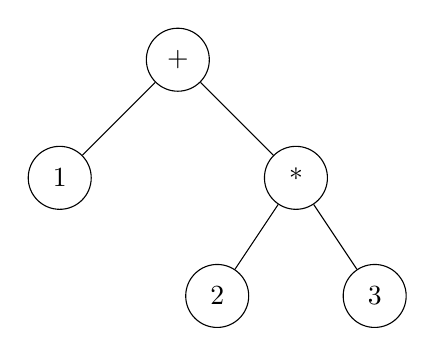
\begin{tikzpicture}[
  level distance=1.5cm,
  level 1/.style={sibling distance=3cm},
  level 2/.style={sibling distance=2cm},
  every node/.style={circle, draw, minimum size=8mm}
]
  \node {+}
    child {node {1}}
    child {node {*}
      child {node {2}}
      child {node {3}}
    };
\end{tikzpicture}
\end{center}

\hypertarget{chapter2-ux3082ux3057ux6587ux6cd5ux306eux968eux5c64ux304cux9006ux3060ux3063ux305fux3089}{%
\subsection{もし文法の階層が逆だったら？}\label{chapter2-ux3082ux3057ux6587ux6cd5ux306eux968eux5c64ux304cux9006ux3060ux3063ux305fux3089}}

以下のような\textbf{誤った}文法を書いたとしましょう：

\begin{verbatim}
// 誤った文法（優先順位が逆）
expr = factor { ('*' | '/') factor };
factor = term { ('+' | '-') term };
term = NUMBER | '(' expr ')';
\end{verbatim}

この場合、\texttt{1+2*3}は\texttt{(1+2)*3}として解析されてしまいます。なぜなら、以下のような解析手順になるからです：

\begin{enumerate}
\def\labelenumi{\arabic{enumi}.}
\tightlist
\item
  \texttt{expr}が最初に\texttt{*}や\texttt{/}を探す
\item
  \texttt{factor}で\texttt{1+2}全体が先に処理される
\item
  その後で\texttt{*3}が処理される
\end{enumerate}

\hypertarget{chapter2-ux6587ux6cd5ux8a2dux8a08ux306eux539fux5247}{%
\subsection{文法設計の原則}\label{chapter2-ux6587ux6cd5ux8a2dux8a08ux306eux539fux5247}}

演算子の優先順位を正しく表現するための原則は以下のようになります：

\begin{enumerate}
\def\labelenumi{\arabic{enumi}.}
\tightlist
\item
  優先順位の低い演算子ほど上位の規則で扱う
\end{enumerate}

\begin{itemize}
\tightlist
\item
  \texttt{+}, \texttt{-}は最上位の\texttt{expr}で
\item
  \texttt{*}, \texttt{/}は中間の\texttt{term}で
\end{itemize}

\begin{enumerate}
\def\labelenumi{\arabic{enumi}.}
\setcounter{enumi}{1}
\tightlist
\item
  同じ優先順位の演算子は同じ規則内で扱う
\end{enumerate}

\begin{itemize}
\tightlist
\item
  \texttt{+}と\texttt{-}は同じ\texttt{expr}内
\item
  \texttt{*}と\texttt{/}は同じ\texttt{term}内
\end{itemize}

\begin{enumerate}
\def\labelenumi{\arabic{enumi}.}
\setcounter{enumi}{2}
\tightlist
\item
  左結合性は繰り返しで表現
\end{enumerate}

\begin{itemize}
\tightlist
\item
  \texttt{\{...\}}による繰り返しが左から右への結合を実現
\end{itemize}

このような階層構造により、パーサーは自然に演算子の優先順位を守りながら解析を進めることができるのです。

\hypertarget{chapter2-ux62bdux8c61ux69cbux6587ux6728}{%
\section{抽象構文木}\label{chapter2-ux62bdux8c61ux69cbux6587ux6728}}
\index{ちゅうしょうこうぶんぎ@抽象構文木}
\index{AST}
\index{ないぶのーど@内部ノード}
\index{はのーど@葉ノード}
\index{ねのーど@根ノード}
\index{ひょうか@評価}

算術式の文法をBNFで表現し、実際に算術式を表す文字列と照合することができました。しかし、これでは文字列が与えられたBNFにマッチするかどうかの判定しかできません。

皆さんおなじみのJSONがそうであるように、実用的には解析した結果を何らかのデータ構造に変換して格納しておく必要があります。そのためのデータ構造が\textbf{抽象構文木}（Abstract
Syntax Tree）です。

抽象構文木とは何でしょうか？今、私達が欲しいのは

\begin{itemize}
\tightlist
\item
  空白や括弧といった余分な情報が含まれず
\item
  演算子の優先順位を表現できる
\end{itemize}

ような構造です。\textbf{抽象構文木}（Abstract Syntax
Tree）は、そのようなニーズを満たすデータ構造です。

抽象構文木は一般には任意個の子を持つ多分木として表現されます。

たとえば、\texttt{1\ +\ 2\ *\ 3}という算術式の抽象構文木は以下のようになります。

\begin{center}
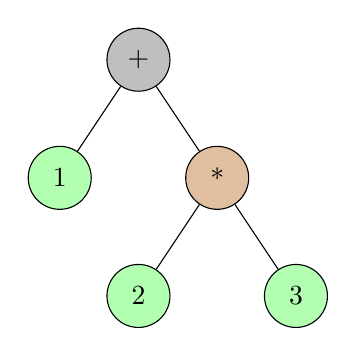
\begin{tikzpicture}[
  level distance=1.5cm,
  sibling distance=2cm,
  every node/.style={circle,draw,minimum size=0.8cm},
  root/.style={fill=gray!50},
  internal/.style={fill=brown!50},
  leaf/.style={fill=green!30}
]
  \node[root] {+}
    child { node[leaf] {1} }
    child { node[internal] {*}
      child { node[leaf] {2} }
      child { node[leaf] {3} }
    };
\end{tikzpicture}
\end{center}

抽象構文木の各ノードは、プログラムの構造を表現するためのデータ構造です。たとえば、\texttt{+}ノードは足し算を表し、\texttt{1}ノードは整数の\texttt{1}を表します。

抽象構文木（AST）では、各ノードはプログラムの構成要素を表し、親子関係によって演算子とその演算対象（オペランド）の関係性を示します。例えば、\texttt{1\ +\ 2}という式では、\texttt{+}が演算子、\texttt{1}と\texttt{2}がオペランドです。抽象構文木には次のようなノードがあります。

\hypertarget{chapter2-ux5185ux90e8ux30ceux30fcux30c9}{%
\subsection{内部ノード}\label{chapter2-ux5185ux90e8ux30ceux30fcux30c9}}

演算子や制御構造など、他のノードを子として持つノードです。
先程の例でいうと、\texttt{+}ノードと\texttt{*}ノードが内部ノードです。

BNFの観点から言えば、内部ノードは主に生成規則の右辺における記号の2つ以上の並びに対応します。

\hypertarget{chapter2-ux8449ux30ceux30fcux30c9}{%
\subsection{葉ノード}\label{chapter2-ux8449ux30ceux30fcux30c9}}

子を持たないノードです。例えば、\texttt{1}や\texttt{2}、\texttt{3}といった数値は葉ノードとなります。
一般的には、リテラルや変数など、それ以上分解できない最小単位のノードが葉ノードとなります。

BNFの観点から言えば、葉ノードは数値リテラルや識別子のような「意味のある値を持つ終端記号」に対応します。一方で、\texttt{+}や\texttt{-}のような演算子は形式上は終端記号ですが、抽象構文木では演算を表す内部ノードのラベルとして現れる点に注意してください。また、\texttt{(}や\texttt{)}、\texttt{,}のような区切りに使われる終端記号は、一般に抽象構文木では消えてしまい、ノードとしては現れません。

\hypertarget{chapter2-ux6839ux30ceux30fcux30c9}{%
\subsection{根ノード}\label{chapter2-ux6839ux30ceux30fcux30c9}}

抽象構文木の最上位に位置するノードです。抽象構文木の根となるノードであり、プログラム全体を表します。数式の例でいえば、全体を表す\texttt{+}ノードが根ノードとなります。
内部ノードと根ノードは排他でないことに注意してください。たとえば、\texttt{+}ノードは内部ノードであり、同時に根ノードでもあります。

\hypertarget{chapter2-ux512aux5148ux9806ux4f4d}{%
\subsection{優先順位}\label{chapter2-ux512aux5148ux9806ux4f4d}}

改めて、先程の抽象構文木を見てみましょう。

\begin{center}
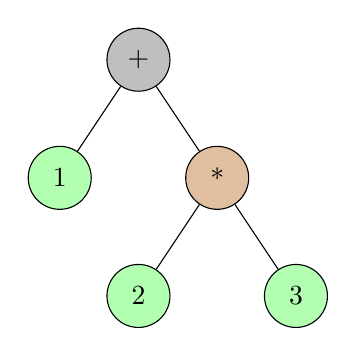
\begin{tikzpicture}[
  level distance=1.5cm,
  sibling distance=2cm,
  every node/.style={circle,draw,minimum size=0.8cm},
  root/.style={fill=gray!50},
  internal/.style={fill=brown!50},
  leaf/.style={fill=green!30}
]
  \node[root] {+}
    child { node[leaf] {1} }
    child { node[internal] {*}
      child { node[leaf] {2} }
      child { node[leaf] {3} }
    };
\end{tikzpicture}
\end{center}

この木構造では、\texttt{+}がルートノードであり、その左の子が\texttt{1}、右の子が\texttt{*}です。\texttt{*}ノードの子として\texttt{2}と\texttt{3}が配置されています。これにより、演算の優先順位が明確に表現されるわけです。

この抽象構文木を見れば、\texttt{1\ +\ (2\ *\ 3)}
という演算順序が表現されており、\texttt{(1\ +\ 2)\ *\ 3}
のような異なる解釈にはならないことが直感的に理解できるでしょう。

\hypertarget{chapter2-ux62bdux8c61ux69cbux6587ux6728ux3092javaux3067ux8868ux73feux3059ux308b}{%
\subsection{抽象構文木をJavaで表現する}\label{chapter2-ux62bdux8c61ux69cbux6587ux6728ux3092javaux3067ux8868ux73feux3059ux308b}}

抽象構文木は視覚的な表現としても便利ですが、その真価はプログラム上で表現・処理することにあります。ここではJavaで表現する方法を紹介します。

\begin{Shaded}
\begin{Highlighting}[]
\CommentTok{// 式を表すインタフェース}
\NormalTok{sealed }\KeywordTok{interface}\NormalTok{ Exp permits Add, Sub, Mul, Div, Num \{\}}
\CommentTok{// 加算を表すレコード}
\CommentTok{// lhs: left{-}hand side（左辺）、rhs: right{-}hand side（右辺）}
\NormalTok{record }\FunctionTok{Add}\NormalTok{(Exp lhs, Exp rhs) }\KeywordTok{implements}\NormalTok{ Exp \{\}}
\CommentTok{// 減算を表すレコード}
\NormalTok{record }\FunctionTok{Sub}\NormalTok{(Exp lhs, Exp rhs) }\KeywordTok{implements}\NormalTok{ Exp \{\}}
\CommentTok{// 乗算を表すレコード}
\NormalTok{record }\FunctionTok{Mul}\NormalTok{(Exp lhs, Exp rhs) }\KeywordTok{implements}\NormalTok{ Exp \{\}}
\CommentTok{// 除算を表すレコード}
\NormalTok{record }\FunctionTok{Div}\NormalTok{(Exp lhs, Exp rhs) }\KeywordTok{implements}\NormalTok{ Exp \{\}}
\CommentTok{// 数値を表すレコード}
\NormalTok{record }\FunctionTok{Num}\NormalTok{(}\DataTypeTok{int}\NormalTok{ value) }\KeywordTok{implements}\NormalTok{ Exp \{\}}
\end{Highlighting}
\end{Shaded}

インタフェース\texttt{Exp}は、抽象構文木のノードを表すインタフェースです。

\texttt{Add}、\texttt{Sub}、\texttt{Mul}、\texttt{Div}、\texttt{Num}は、それぞれ加算、減算、乗算、除算、数値を表すレコードです。これによって、抽象構文木をJavaで表現することができます。

試しに\texttt{1\ +\ 2\ *\ 3}の抽象構文木をJavaで表現してみましょう。

\begin{Shaded}
\begin{Highlighting}[]
\CommentTok{// 1 + 2 * 3}
\NormalTok{Exp exp = }\KeywordTok{new} \FunctionTok{Add}\NormalTok{(}
  \KeywordTok{new} \FunctionTok{Num}\NormalTok{(}\DecValTok{1}\NormalTok{), }\KeywordTok{new} \FunctionTok{Mul}\NormalTok{(}\KeywordTok{new} \FunctionTok{Num}\NormalTok{(}\DecValTok{2}\NormalTok{), }\KeywordTok{new} \FunctionTok{Num}\NormalTok{(}\DecValTok{3}\NormalTok{))}
\NormalTok{);}
\end{Highlighting}
\end{Shaded}

各クラスのインスタンスを作成することで、抽象構文木を表現することができます。

\hypertarget{chapter2-ux62bdux8c61ux69cbux6587ux6728ux3092ux8a55ux4fa1ux3059ux308b}{%
\subsection{抽象構文木を評価する}\label{chapter2-ux62bdux8c61ux69cbux6587ux6728ux3092ux8a55ux4fa1ux3059ux308b}}

構文解析が完了して抽象構文木が得られると、その先にはどのような可能性が広がるのでしょうか。実は、抽象構文木さえ作ってしまえば、それを活用して様々なことができるようになります。その一例として、ここでは抽象構文木を「評価」して計算結果を得る方法を紹介します。

抽象構文木を作成するだけでは、プログラムの実行結果を得ることはできません。抽象構文木を評価するためには、再帰的な処理を行うことが必要です。抽象構文木を辿りながら、各ノードの演算を行うことで、プログラムの実行結果を得ることができます。

以下は、算術式の抽象構文木を評価するJavaのコード例です。

\begin{Shaded}
\begin{Highlighting}[]
\DataTypeTok{int} \FunctionTok{eval}\NormalTok{(Exp e) \{}
  \KeywordTok{return} \KeywordTok{switch}\NormalTok{(e)\{}
    \KeywordTok{case}\NormalTok{ Num t {-}\textgreater{} t.}\FunctionTok{value}\NormalTok{();}
    \KeywordTok{case}\NormalTok{ Add t {-}\textgreater{} }\FunctionTok{eval}\NormalTok{(t.}\FunctionTok{lhs}\NormalTok{()) + }\FunctionTok{eval}\NormalTok{(t.}\FunctionTok{rhs}\NormalTok{());}
    \KeywordTok{case}\NormalTok{ Sub t {-}\textgreater{} }\FunctionTok{eval}\NormalTok{(t.}\FunctionTok{lhs}\NormalTok{()) {-} }\FunctionTok{eval}\NormalTok{(t.}\FunctionTok{rhs}\NormalTok{());}
    \KeywordTok{case}\NormalTok{ Mul t {-}\textgreater{} }\FunctionTok{eval}\NormalTok{(t.}\FunctionTok{lhs}\NormalTok{()) * }\FunctionTok{eval}\NormalTok{(t.}\FunctionTok{rhs}\NormalTok{());}
    \KeywordTok{case}\NormalTok{ Div t {-}\textgreater{} \{}
      \DataTypeTok{int}\NormalTok{ divisor = }\FunctionTok{eval}\NormalTok{(t.}\FunctionTok{rhs}\NormalTok{()); }\CommentTok{// 先に右辺を評価}
      \KeywordTok{if}\NormalTok{(divisor == }\DecValTok{0}\NormalTok{) \{ }\CommentTok{// 評価結果でゼロチェック}
        \KeywordTok{throw} \KeywordTok{new} \BuiltInTok{ArithmeticException}\NormalTok{(}\StringTok{"division by zero"}\NormalTok{);}
\NormalTok{      \}}
\NormalTok{      yield }\FunctionTok{eval}\NormalTok{(t.}\FunctionTok{lhs}\NormalTok{()) / divisor; }\CommentTok{// 左辺を評価して除算}
\NormalTok{    \}}
\NormalTok{  \};}
\NormalTok{\}}
\end{Highlighting}
\end{Shaded}

ノードの種類に応じてswitch式で処理を分岐しています：

\begin{itemize}
\tightlist
\item
  \texttt{Num}ノードの場合: 格納されている数値 \texttt{t.value()}
  をそのまま返します。これが再帰のベースケースとなります。
\item
  \texttt{Add}ノードの場合: 左の子 \texttt{t.lhs()} と右の子
  \texttt{t.rhs()} をそれぞれ再帰的に \texttt{eval}
  し、その結果を足し算します。
\item
  \texttt{Sub}、\texttt{Mul}ノードの場合: \texttt{Add}
  と同様に、左右の子を再帰的に評価し、それぞれの演算を行います。
\item
  \texttt{Div}ノードの場合: まず右の子（除数）を \texttt{eval}
  し、その結果が0であれば \texttt{ArithmeticException}
  をスローします。0でなければ、次に左の子（被除数）を \texttt{eval}
  し、除算の結果を返します。ゼロ除算チェックは、実際の計算を行う前に行うことが重要です。また、\texttt{eval(t.rhs())}
  を2回呼び出すのを避けるため、一度評価した結果を変数に格納しています。
\end{itemize}

この\texttt{eval}メソッドの動作を \texttt{1\ +\ 2\ *\ 3} の抽象構文木
\texttt{new\ Add(new\ Num(1),\ new\ Mul(new\ Num(2),\ new\ Num(3)))}
で追ってみましょう。

\begin{itemize}
\tightlist
\item
  \texttt{eval(new\ Add(new\ Num(1),\ new\ Mul(new\ Num(2),\ new\ Num(3))))}
  が呼び出される。

  \begin{itemize}
  \tightlist
  \item
    \texttt{Add}ケースにマッチ。
  \item
    \texttt{eval(t.lhs())} つまり \texttt{eval(new\ Num(1))}
    が呼び出される。

    \begin{itemize}
    \tightlist
    \item
      \texttt{Num}ケースにマッチ。\texttt{1} を返す。
    \end{itemize}
  \item
    \texttt{eval(t.rhs())} つまり
    \texttt{eval(new\ Mul(new\ Num(2),\ new\ Num(3)))} が呼び出される。

    \begin{itemize}
    \tightlist
    \item
      \texttt{Mul}ケースにマッチ。
    \item
      \texttt{eval(t.lhs())} つまり \texttt{eval(new\ Num(2))}
      が呼び出される。

      \begin{itemize}
      \tightlist
      \item
        \texttt{Num}ケースにマッチ。\texttt{2} を返す。
      \end{itemize}
    \item
      \texttt{eval(t.rhs())} つまり \texttt{eval(new\ Num(3))}
      が呼び出される。

      \begin{itemize}
      \tightlist
      \item
        \texttt{Num}ケースにマッチ。\texttt{3} を返す。
      \end{itemize}
    \item
      \texttt{2\ *\ 3} の結果である \texttt{6} を返す。
    \end{itemize}
  \item
    \texttt{1\ +\ 6} の結果である \texttt{7} を返す。
  \end{itemize}
\end{itemize}

このように抽象構文木を再帰的に辿ることで、式の評価が実現されます。

\texttt{Div}
の場合のゼロ除算エラー処理は、プログラムの実行時エラーを防ぐために不可欠です。他の演算（\texttt{Add},
\texttt{Sub},
\texttt{Mul}）では、Javaの整数演算がオーバーフローする可能性はありますが、\texttt{ArithmeticException}
のような実行時例外を直接引き起こす「不正な演算」は（ゼロ除算ほど明確には）定義されていないため、ここでは特にエラー処理を加えていません（もちろん、より堅牢な電卓を作る場合はオーバーフロー検知なども考慮に入れるべきです）。

\texttt{eval}メソッドを使うことで、次のように抽象構文木を評価することができます。

\begin{Shaded}
\begin{Highlighting}[]
\CommentTok{// 1 + 2 * 3}
\NormalTok{Exp exp = }\KeywordTok{new} \FunctionTok{Add}\NormalTok{(}
  \KeywordTok{new} \FunctionTok{Num}\NormalTok{(}\DecValTok{1}\NormalTok{), }\KeywordTok{new} \FunctionTok{Mul}\NormalTok{(}\KeywordTok{new} \FunctionTok{Num}\NormalTok{(}\DecValTok{2}\NormalTok{), }\KeywordTok{new} \FunctionTok{Num}\NormalTok{(}\DecValTok{3}\NormalTok{))}
\NormalTok{);}
\FunctionTok{eval}\NormalTok{(exp); }\CommentTok{// 7}
\end{Highlighting}
\end{Shaded}

抽象構文木をデータとして表現することで、プログラムの構造を簡単に解析することができるのです。

\hypertarget{chapter2-ux307eux3068ux3081}{%
\section{まとめ}\label{chapter2-ux307eux3068ux3081}}

この章では、算術式の文法を例題としてBNFについて紹介し、BNFに基づいて算術式を解析する方法の概要について説明しました。また、抽象構文木についても紹介し、抽象構文木をJavaで表現する方法と、抽象構文木を評価する方法について説明しました。

しかし、今のままではBNFに基づく「構文解析器」は与えられた文字列が文法にマッチするかどうかを判定するだけで、抽象構文木を生成することができません。次章では、ここで学んだBNFの考え方を応用して、実際にJavaで動作するJSONの構文解析器を実装し、JSONの抽象構文木を生成する方法について詳しく説明します。
